\documentclass[UTF8,fontset=none,a4paper]{ctexart}

\usepackage{fontspec}
\setmainfont{Arial}
\setsansfont{Arial}
\setCJKmainfont{Hiragino Sans GB}
\setCJKsansfont{Hiragino Sans GB}
\renewcommand{\familydefault}{\sfdefault}

\usepackage[
  top=18mm,
  bottom=18mm,
  left=12mm,
  right=12mm,
  headheight=12pt,
  headsep=3mm,
  footskip=8mm
]{geometry}
\usepackage{graphicx}
\usepackage{booktabs}
\usepackage{tabularx}
\usepackage{array}
\usepackage[table]{xcolor}
\usepackage{tikz}
\usetikzlibrary{arrows.meta,positioning,fit}
\usepackage[numbers,sort&compress]{natbib}
\usepackage{hyperref}
\usepackage{microtype}
\usepackage{enumitem}
\usepackage{caption}
\usepackage{fancyhdr}
\usepackage{ragged2e}

\definecolor{blue}{HTML}{2563EB}
\definecolor{bluepale}{HTML}{EFF6FF}
\definecolor{green}{HTML}{15803D}
\definecolor{greenpale}{HTML}{F0FDF4}
\definecolor{orange}{HTML}{D97706}
\definecolor{orangepale}{HTML}{FFF7ED}
\definecolor{ink}{HTML}{0F172A}
\definecolor{muted}{HTML}{475569}
\definecolor{line}{HTML}{CBD5E1}
\definecolor{surface}{HTML}{F8FAFC}

\hypersetup{
  colorlinks=true,
  linkcolor=blue,
  citecolor=blue,
  urlcolor=blue,
  pdftitle={Loreley: Evolution Dynamics Technical Report},
  pdfauthor={Mohan Chen}
}

\pagestyle{fancy}
\fancyhf{}
\fancyhead[L]{\color{muted}\footnotesize LORELEY 技术报告}
\fancyhead[R]{\color{muted}\footnotesize 进化动力学视角}
\fancyfoot[C]{\color{muted}\footnotesize \thepage\ / 4}
\renewcommand{\headrulewidth}{0.35pt}
\renewcommand{\footrulewidth}{0pt}
\setlength{\parindent}{0pt}
\setlength{\parskip}{3.2pt}
\setlength{\emergencystretch}{2em}
\setlist[itemize]{leftmargin=1.2em,itemsep=1pt,topsep=2pt,parsep=0pt}
\captionsetup{font=small,labelfont=bf,skip=3pt}
\newcolumntype{Y}{>{\RaggedRight\arraybackslash}X}
\newcolumntype{C}[1]{>{\centering\arraybackslash}p{#1}}

\newcommand{\pagetitle}[2]{%
  {\color{blue}\fontsize{11}{12}\selectfont\bfseries #1}\par
  {\color{ink}\fontsize{20}{22}\selectfont\bfseries #2}\vspace{3pt}\par
  {\color{line}\rule{\textwidth}{0.65pt}}\vspace{4pt}
}

\newcommand{\metriccard}[3]{%
  \begin{minipage}[t][19mm][c]{0.235\textwidth}
    \centering
    {\color{#3}\fontsize{20}{21}\selectfont\bfseries #1}\par
    {\color{muted}\scriptsize #2}
  \end{minipage}%
}

\newcommand{\callout}[2]{%
  \colorbox{bluepale}{%
    \parbox{\dimexpr\linewidth-2\fboxsep\relax}{%
      \vspace{2pt}{\color{blue}\bfseries #1}\quad #2\vspace{2pt}%
    }%
  }%
}

\newcommand{\decisionbox}[3]{%
  \begin{minipage}[t]{0.315\textwidth}
    \colorbox{#1}{\parbox{\dimexpr\linewidth-2\fboxsep\relax}{%
      \vspace{3pt}{\bfseries #2}\par\small #3\vspace{3pt}}}
  \end{minipage}%
}

\begin{document}
\zihao{-5}

% -----------------------------------------------------------------------------
% Page 1
% -----------------------------------------------------------------------------
\thispagestyle{fancy}
\vspace*{-3mm}
{\color{ink}\fontsize{25}{27}\selectfont\bfseries
Loreley：完整代码仓库的并行、多分支进化}\par
\vspace{2pt}
{\color{muted}\fontsize{12}{14}\selectfont
墙钟时间与长周期搜索中的质量演化}\hfill
{\small Mohan Chen · 2026-09}\par
\vspace{5pt}

\colorbox{surface}{\parbox{\dimexpr\textwidth-2\fboxsep\relax}{%
\vspace{3pt}
\metriccard{2.78$\times$}{顺序冠军 / QD 的 48 任务\par 配对耗时几何均值}{blue}\hfill
\metriccard{7/7}{QD 完成 48 个任务时\par 全部区组均领先}{green}\hfill
\metriccard{6/7}{最终达到 +0.50\%\par 门槛的 QD 区组}{blue}\hfill
\metriccard{3--42}{保留分支到最终后代的\par 任务间隔}{orange}
\vspace{3pt}}}

\vspace{6pt}
\callout{主要结果}{Loreley QD 同时推进多个分支，并把通过评估的中间状态留作后续父代。它比顺序冠军更早找到达到门槛的候选；按相同 48 个任务比较，顺序冠军的终点均值略高。}

\vspace{6pt}
{\color{ink}\large\bfseries 三种策略的谱系关系}\par
\vspace{3pt}
\begin{center}
\begin{tikzpicture}[
  x=1mm,
  y=1mm,
  root/.style={
    circle,minimum size=4.6mm,inner sep=0pt,draw=ink,fill=ink,
    text=white,font=\tiny\bfseries
  },
  state/.style={
    circle,minimum size=3.8mm,inner sep=0pt,line width=0.65pt
  },
  independent/.style={state,draw=muted,fill=white},
  qd/.style={state,draw=blue,fill=white},
  champion/.style={state,draw=orange,fill=white},
  stopped/.style={state,draw=line,fill=surface},
  gene/.style={
    -{Latex[length=1.2mm,width=0.9mm]},line width=0.65pt,draw=muted
  },
  stoppedgene/.style={gene,draw=line},
  paneltitle/.style={font=\small\bfseries,text=ink,align=center},
  panelnote/.style={font=\scriptsize,text=muted,align=center}
]
  % Independent Root
  \begin{scope}[shift={(0,0)}]
    \path[draw=line,fill=surface,rounded corners=2mm]
      (0,0) rectangle (57,32);
    \node[paneltitle] at (28.5,27.5) {从根独立};
    \node[root] (ir-root) at (10,16) {根};
    \node[independent] (ir-a) at (44,10) {};
    \node[independent] (ir-b) at (44,16) {};
    \node[independent] (ir-c) at (44,22) {};
    \draw[gene] (ir-root) -- (ir-a);
    \draw[gene] (ir-root) -- (ir-b);
    \draw[gene] (ir-root) -- (ir-c);
    \node[panelnote] at (28.5,4) {候选都从同一根提交出发};
  \end{scope}

  % Loreley QD
  \begin{scope}[shift={(61,0)}]
    \path[draw=blue,fill=bluepale,rounded corners=2mm]
      (0,0) rectangle (57,32);
    \node[paneltitle] at (28.5,27.5) {Loreley QD};
    \node[root] (qd-root) at (7,16) {根};
    \node[qd] (qd-a) at (18,21) {};
    \node[qd] (qd-b) at (18,11) {};
    \node[qd] (qd-c) at (31,23) {};
    \node[stopped] (qd-d) at (31,17) {};
    \node[qd] (qd-e) at (32,10) {};
    \node[qd] (qd-f) at (47,21) {};
    \node[qd] (qd-g) at (47,10) {};
    \draw[gene,draw=blue] (qd-root) -- (qd-a);
    \draw[gene,draw=blue] (qd-root) -- (qd-b);
    \draw[gene,draw=blue] (qd-a) -- (qd-c);
    \draw[stoppedgene] (qd-a) -- (qd-d);
    \draw[gene,draw=blue] (qd-b) -- (qd-e);
    \draw[gene,draw=blue] (qd-c) -- (qd-f);
    \draw[gene,draw=blue] (qd-e) -- (qd-g);
    \node[panelnote] at (28.5,4) {多个保留分支可以继续};
  \end{scope}

  % Sequential Champion
  \begin{scope}[shift={(122,0)}]
    \path[draw=orange,fill=orangepale,rounded corners=2mm]
      (0,0) rectangle (57,32);
    \node[paneltitle] at (28.5,27.5) {顺序冠军};
    \node[root] (sc-root) at (7,16) {根};
    \node[champion] (sc-a) at (19,16) {};
    \node[champion] (sc-b) at (31,16) {};
    \node[champion] (sc-c) at (45,16) {};
    \node[stopped] (sc-d) at (19,9.5) {};
    \node[stopped] (sc-e) at (31,22.5) {};
    \draw[gene,draw=orange] (sc-root) -- (sc-a);
    \draw[gene,draw=orange] (sc-a) -- (sc-b);
    \draw[gene,draw=orange] (sc-b) -- (sc-c);
    \draw[stoppedgene] (sc-root) -- (sc-d);
    \draw[stoppedgene] (sc-a) -- (sc-e);
    \node[panelnote] at (28.5,4) {只有当前冠军分支继续};
  \end{scope}
\end{tikzpicture}
\end{center}
\vspace{3pt}

{\color{ink}\large\bfseries 三种策略的动力学差别}\par
\vspace{2pt}
{\small
\setlength{\tabcolsep}{5pt}
\renewcommand{\arraystretch}{1.18}
\begin{tabularx}{\textwidth}{@{}Y C{17mm} C{20mm} C{25mm} C{27mm} C{20mm}@{}}
\toprule
策略 & 并行候选 & 跨代累积 & 搜索时间中位数 & 48 任务平均提升 & 终点达标区组 \\
\midrule
从根独立 & 是 & 否 & 3.66 h & +0.50\% & 2/7 \\
\rowcolor{bluepale}
\textbf{Loreley QD} & \textbf{是} & \textbf{是} & \textbf{3.75 h} & \textbf{+0.82\%} & \textbf{6/7} \\
顺序冠军 & 否 & 是 & 11.65 h & +0.96\% & 7/7 \\
\bottomrule
\end{tabularx}}

\vspace{7pt}
\begin{minipage}[t]{0.485\textwidth}
{\color{ink}\large\bfseries 系统流程}\par
\small
编码智能体从可构建的仓库提交出发，在隔离的工作树中完成跨文件修改。项目评估器检查构建、测试和编辑范围，并记录多个性能指标。只有通过门槛的提交进入档案；每个 Git 提交既保存代码状态，也记录谱系关系。\par
档案中的提交可以再次被选作父代或参考分支，因此每次保留都会影响后续候选的生成路径。
\end{minipage}\hfill
\begin{minipage}[t]{0.485\textwidth}
{\color{ink}\large\bfseries 对照设置}\par
\small
Zstandard 实验包含 7 个配对区组。每种策略在每组运行 48 个候选任务，共 1,008 个任务。三种策略使用相同的初始提交、智能体路由、评估器和候选选择规则，只改变父代选择和调度方式。分别在第 8、16、24、32、40 和 48 个任务后，用验证集选择当前候选，再在留出集上测量。\par
按相同任务数比较搜索效率；按相同墙钟时间比较交付速度。
\end{minipage}

\clearpage

% -----------------------------------------------------------------------------
% Page 2
% -----------------------------------------------------------------------------
\pagetitle{01 / 墙钟时间}{更快拿到可用候选}

\begin{center}
  % Use the 300 dpi render to avoid platform-specific TTC font subsets.
  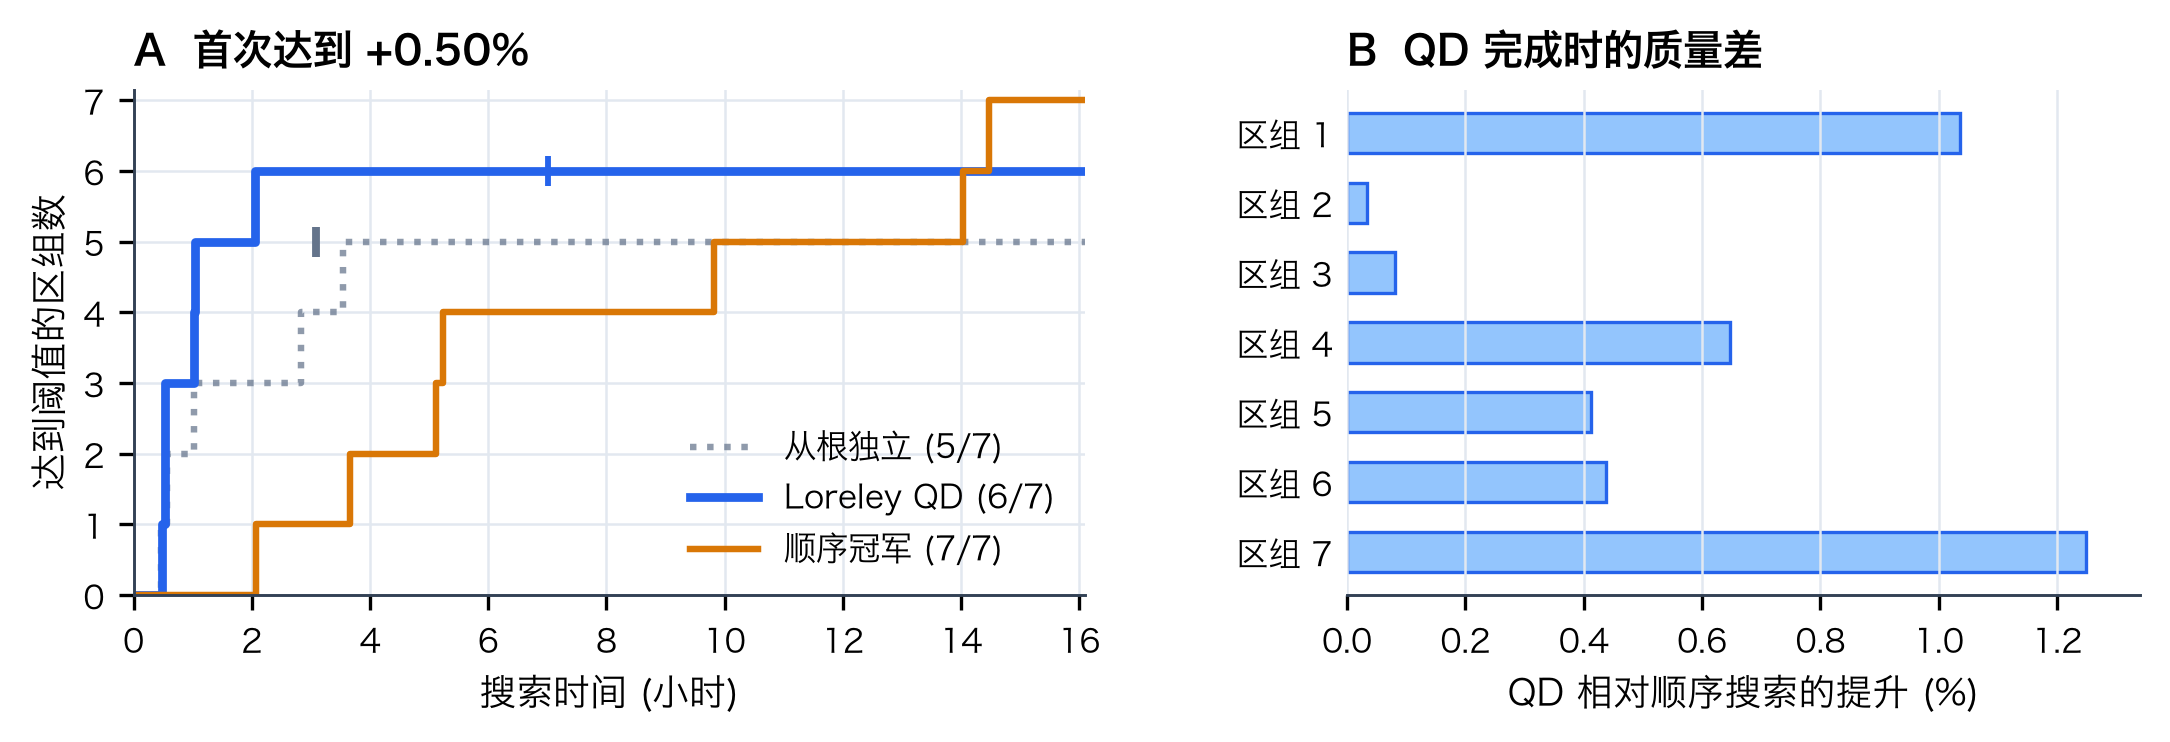
\includegraphics[width=0.985\textwidth]{figures/quality_time.png}
\end{center}
\vspace{2pt}

\begin{minipage}[t]{0.48\textwidth}
{\color{ink}\large\bfseries 达到 $+0.50\%$ 所需时间}\par
\small
实验将 $+0.50\%$ 压缩吞吐提升设为有效改进门槛。首次达到门槛的时间取自各组已有检查点：
\vspace{3pt}

\begin{tabularx}{\linewidth}{@{}Y r r@{}}
\toprule
策略 & 达标区组 & 首次达标时间 \\
\midrule
\textbf{Loreley QD} & \textbf{6/7} & \textbf{中位数 0.78 h} \\
顺序冠军 & 7/7 & 中位数 5.23 h \\
\bottomrule
\end{tabularx}

\vspace{3pt}
在两种策略均达到门槛的 6 个区组中，QD 都更快。顺序冠军与 QD 的首次达标时间比几何均值为 $6.76\times$。QD 的范围为 0.48--2.05 小时，顺序冠军为 2.08--14.46 小时。

\vspace{5pt}
{\color{ink}\bfseries 关键路径决定时间差}\par
QD 同时运行 4 个候选，有效并行度中位数为 3.37；顺序冠军每次只运行 1 个，有效并行度为 0.99。各策略在各区组内的累计排队时间约为 3--7 分钟，无法解释两者的小时级差距。QD 可同时推进多个分支，顺序冠军则受单条依赖链限制。
\end{minipage}\hfill
\begin{minipage}[t]{0.48\textwidth}
{\color{ink}\large\bfseries 按任务数和按时间比较}\par
\small
\colorbox{orangepale}{\parbox{\dimexpr\linewidth-2\fboxsep\relax}{%
\vspace{3pt}\textbf{固定 48 个任务：顺序冠军终点更高。}\par
留出集平均提升分别为顺序冠军 $+0.96\%$、QD $+0.82\%$、从根独立 $+0.50\%$。在固定任务数口径下，顺序冠军的终点均值最高。\vspace{3pt}}}

\vspace{5pt}
\colorbox{bluepale}{\parbox{\dimexpr\linewidth-2\fboxsep\relax}{%
\vspace{3pt}\textbf{固定 QD 的完成时间：全部 7 组由 QD 领先。}\par
QD 完成 48 个任务时，顺序冠军最近的检查点分别为：4 组第 8 个任务、2 组第 16 个任务、1 组第 24 个任务。此时 QD 在全部 7 组中得分更高，逐组优势的中位数为 $+0.44\%$。\vspace{3pt}}}

\vspace{5pt}
\colorbox{greenpale}{\parbox{\dimexpr\linewidth-2\fboxsep\relax}{%
\vspace{3pt}\textbf{在给定时间内，QD 交付更好的候选。}\par
QD 的总耗时接近从根独立，同时能够跨代累积修改。交付时间受限时，墙钟时间下的质量曲线比单看第 48 个任务后的终点更有参考价值。\vspace{3pt}}}
\end{minipage}

\vspace{7pt}
{\color{muted}\scriptsize
墙钟时间根据 1,008 条候选任务时间戳重建，仅统计候选搜索。每个检查点先在验证集选择候选，再在留出集测量压缩吞吐；检查点之间不插值。竖线表示 48 个任务内未达到门槛。}

\clearpage

% -----------------------------------------------------------------------------
% Page 3
% -----------------------------------------------------------------------------
\pagetitle{02 / 长周期搜索}{后半程仍有新候选}

\begin{center}
  % Use the 300 dpi render to avoid platform-specific TTC font subsets.
  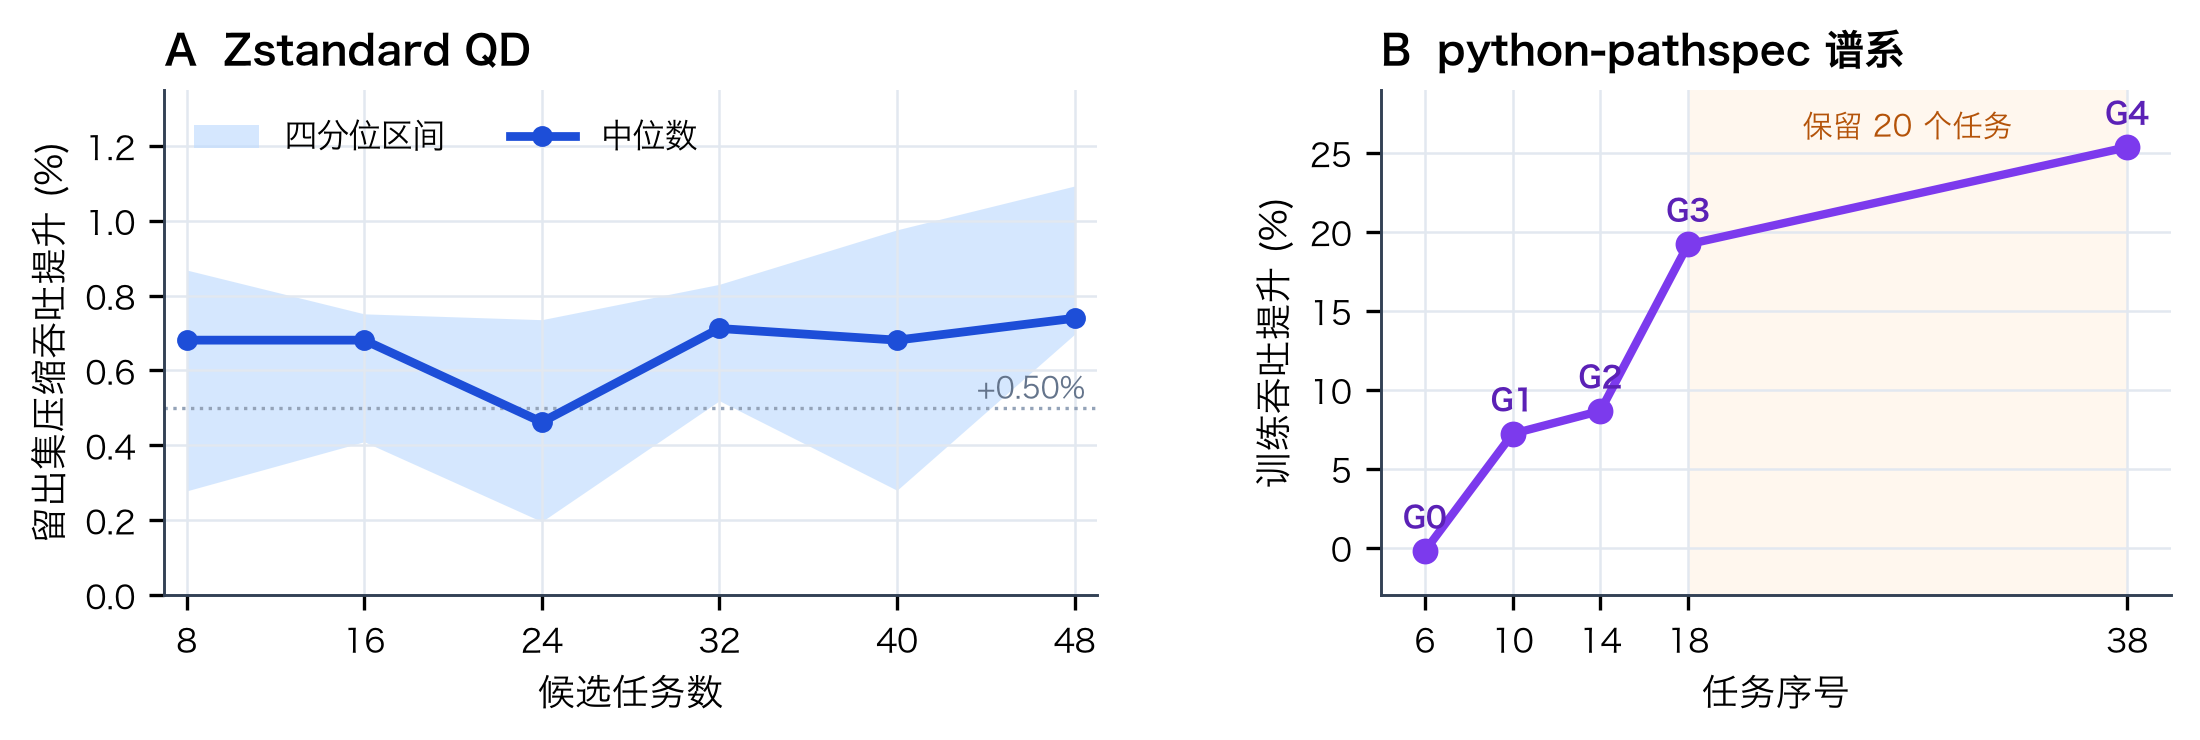
\includegraphics[width=0.985\textwidth]{figures/job_dynamics.png}
\end{center}
\vspace{3pt}

\colorbox{surface}{\parbox{\dimexpr\textwidth-2\fboxsep\relax}{%
\vspace{2pt}
\metriccard{20}{不同主父代 / 区组\par 中位数；范围 15--23}{blue}\hfill
\metriccard{5.5}{再次选择父代的\par 任务间隔中位数}{blue}\hfill
\metriccard{5--9}{各区组达到的\par 最大代数}{green}\hfill
\metriccard{3--42}{保留分支到最终后代的\par 任务间隔}{orange}
\vspace{2pt}}}

\vspace{5pt}

\begin{minipage}[t]{0.48\textwidth}
{\color{ink}\large\bfseries 第 24--48 个任务仍有改进}\par
\small
从第 24 个到第 48 个任务，QD 入选候选在留出集上的平均提升从 $+0.47\%$ 增至 $+0.82\%$，中位数从 $+0.46\%$ 增至 $+0.74\%$；5/7 组上升，2/7 组持平。三个最终候选分别到第 26、38 和 43 个任务才出现。\par
在 220 个任务的 Zstandard 长周期运行中，前 128 个任务的每个连续 16 任务区间都有新候选入档；第 129--220 个任务又有 15 次入档。第 4 代候选 \texttt{fe39bee8} 最早出现在第 57 个任务，既有留出集提升为 $+1.17\%$。
\end{minipage}\hfill
\begin{minipage}[t]{0.48\textwidth}
{\color{ink}\large\bfseries 档案如何延长有效搜索}\par
\small
MAP-Elites 仅让同一行为单元内的候选相互竞争，因此暂时未成为全局最优的状态仍可作为后续父代\citep{mouret2015mapelites}。Loreley 在每个单元保留局部 Pareto 前沿，使压缩、解压和最坏单元性能之间的不同权衡得以延续\citep{pierrot2022mome}。\par
Qian 等人在两类组合优化问题上证明：跨单元保留中间状态可使 MAP-Elites 达到多项式期望时间，而全局竞争的进化算法在部分实例上需要指数期望时间\citep{qian2024qdhelpful}。Loreley 的谱系记录显示，非领先分支在间隔多个任务后仍会被重新选中，并产生更好的后代。
\end{minipage}

\vspace{7pt}
\callout{Pathspec 谱系}{该分支在第 18 个任务达到 $1.19\times$ 后被保留。随后 20 个任务从其他分支出发；第 38 个任务重新选中该分支，并产生 $1.25\times$ 的第 4 代候选，参考工作负载提升 $+25.14\%$。}

\clearpage

% -----------------------------------------------------------------------------
% Page 4
% -----------------------------------------------------------------------------
\pagetitle{03 / 应用}{综合看墙钟时间与长期收益}

{\color{ink}\large\bfseries 三个完整仓库上的能力结果}\par
\small
\setlength{\tabcolsep}{5pt}
\renewcommand{\arraystretch}{1.18}
\begin{tabularx}{\textwidth}{@{}Y C{20mm} C{23mm} C{35mm} Y@{}}
\toprule
目标 & 任务数 & 最终代数 & 最终候选结果 & 搜索过程 \\
\midrule
\texttt{markdown-it-py} & 64 & 第 4 代 & 独立验证 $+6.75\%$ & 第 7/12/14/26 个任务逐代累积修改 \\
\texttt{python-pathspec} & 64 & 第 4 代 & 参考负载 $+25.14\%$ & 第 18 个任务保留分支，第 38 个任务继续 \\
Zstandard（长周期） & 220 & 第 4 代 & 既有留出集 $+1.17\%$；新留出集 $+0.89\%$ & 第 57 个任务出现候选；后程仍有 15 次入档 \\
\bottomrule
\end{tabularx}

\vspace{7pt}
{\color{ink}\large\bfseries 对工程决策的影响}\par
\vspace{3pt}
\decisionbox{bluepale}{1. 同时报告达标时间}{候选生成和评估可并行时，QD 避免把所有任务排在单条冠军链上。在本实验中，QD 更早达到 $+0.50\%$ 门槛；到其完成 48 个任务时，7 个区组均领先顺序冠军。}\hfill
\decisionbox{greenpale}{2. 记录分支重访}{评估档案时，应记录父代选择次数、分支重访间隔、最终候选首次出现的任务编号，以及检查点之间的提升。}\hfill
\decisionbox{orangepale}{3. 分别比较任务数与时间}{固定 48 个任务时，顺序冠军的终点均值最高；固定 QD 的完成时间时，QD 在全部 7 组领先。两个口径需要同时报告。}

\vspace{7pt}
\begin{minipage}[t]{0.485\textwidth}
{\color{ink}\large\bfseries 适用条件}\par
\small
\begin{itemize}
  \item 单个候选生成或评估需要数分钟，并且可安全并行运行至少 3--4 个候选；
  \item 优化依赖多代、跨文件的兼容修改；
  \item 正确性、资源与性能约束可由项目评估器统一检查；
  \item 需要保留完整 Git 状态，方便复现、回滚和跨分支组合。
\end{itemize}
\end{minipage}\hfill
\begin{minipage}[t]{0.485\textwidth}
{\color{ink}\large\bfseries 总结}\par
\small
Loreley 将并行候选生成与可重访的多分支档案结合起来。并行调度缩短了达到有效改进所需的墙钟时间；档案保留暂时未领先的中间状态，使其能在后续任务中重新成为父代并继续演化。\par
实验中，QD 更早达到有效改进门槛，并在相同墙钟时间内交付更好的候选。搜索周期延长后，后半程仍有候选入档，保留分支也能跨越多个任务产生更好的后代。Loreley 的优势集中在两点：更快取得可用结果，以及让长周期搜索继续产生增益。
\end{minipage}

\vspace{6pt}
\colorbox{surface}{\parbox{\dimexpr\textwidth-2\fboxsep\relax}{%
\scriptsize\textbf{数据来源。}
Zstandard 对照记录、质量--时间重建结果，以及三个仓库的长周期运行记录。复算脚本覆盖 126 次检查点选择、终点统计和谱系计数。}}

\vspace{3pt}
{\footnotesize
\setlength{\bibsep}{0pt}
\bibliographystyle{abbrvnat}
\bibliography{references}}

\end{document}
